\chapter{Introduction}
As the name suggests the purpose of this chapter is to introduce our work. It begins by explaining the background for the thesis and introducing the context of study. It then presents the research questions and ends with the thesis outline.

\section{Background}
The elderly population is in a constant rise, currently 15\% of the Norwegian population is above the age of 65. By the turn of the century, the elderly population in Norway is estimated to double~\cite{elder}. After 2025, a great increase in the population above the age of 80 is expected. The \gls{niph} reports that two out of three above the age of 75 consider themselves having ``good health'', but only a third preserve this level of health until death~\cite{elder}. The amount of time adults spend in a sedentary position has increased over the last 30 years. The reasons for this are many, but increased use of technology and ease of transport are one of the main factors~\cite{sedentaryBehaviour}.

With such predictions the Norwegian government formed a committee known as \gls{hu} to investigate the current situation and suggest solutions for accommodating the increase in the percentage of elderly~\cite{haagen}. One of the conclusions in the report was that too little of today's technology is incorporated as welfare technology for the elderly. A Danish report refereed to by \gls{hu} states that around 20\% of the tasks performed by healthcare personnel could be completely or partly replaced by technology~\cite{kmd}. 

Recent studies on the activity level of adults and elderly in Norway show that only one in five reach the national goal of 30 minutes of activity each day~\cite{fysiskAktivitet2009}. Increasing the overall activity level of elderly is one of the main foci in the \gls{hu} report. To handle the rising percentage of elderly in the population, \gls{hu} suggests a national three step program that focuses on using welfare technology to diminish falls, social isolation and cognitive failure, thus improving the overall quality of life for the elder population as well as reducing the workload for health care personnel. Step 3 states:

\begin{quote}
\textit{Opt on technology that stimulates, activates and structures daily life}~\cite[page 120]{haagen}
\end{quote}

We wish to address step 3 in the national program through the use of Personal Informatics (PI) technology. \gls{pi} technology is a set of tools that individuals can use to gather quantitative data about themselves for the purpose of self-reflection and self-monitoring. By allowing physiotherapists to collect patient data from an activity monitor and visualizing user patterns, we hope to bring awareness to their activity levels, and identify periods of long sedentary time. The data can in addition be utilized in consultation with health care personnel and rehabilitation facilities, to improve treatment and motivation of patients.

%Burde kanskje kommentere bildet i teksten og ikke bare under bildet?

\begin{figure}[h!]
	\centering
		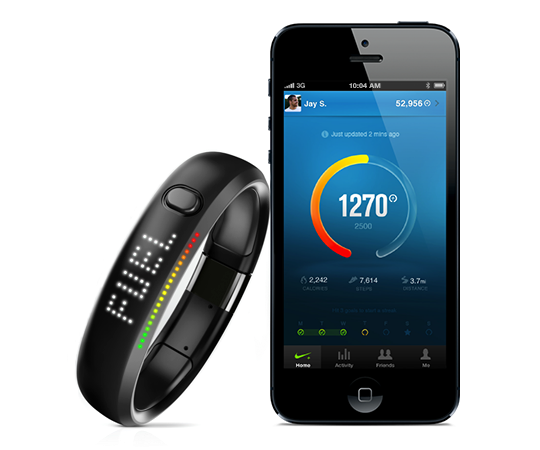
\includegraphics[width=0.6\textwidth]{nikeFuelband.png}
		\caption{\footnotesize A Nike+ Fuelband synced up to an iPhone. This is just one of many \gls{pi} devices available.}
		\label{fig:nikeFuelbandPhone}
\end{figure}

\section{Context of Study}
A large EU project known as FARSEEING is currently in progress. FARSEEING is a collaboration between ten partners in five EU countries and is funded by the European Commission. The aim is to create a thematic network that promotes healthy and independent living for the elderly. FARSEEING wishes to improve fall prediction and prevention, support older adults through technology, and use unique proactive opportunities to keep adults in their own environment.

Our work is not a deliverable in the FARSEEING project, but our advisor and the people we have been in contact with are a part of the project. This leads to a certain influence by the agenda of the FARSEEING project, and we hope that some of our work will aid them in the future.

A practical approach is taken and the entire FARSEEING project is divided into work packages which combined expand the research, technological development and overall knowledge in this area \cite{farseeing}. The \gls{ntnu} is responsible for Work Package 5 and the overall objective for FARSEEING is to develop and validate feasible telemedicine service models for detection of accidental falls, fall risk assessment and exercise counselling \cite{wp5}. The service models should not be dependent on a specific technological platforms or sensor systems used to collect and disseminate data. The overall objective has been divided into three different domains. The second domain is partly relevant to the work performed in this thesis.

\begin{quote}
\textit{To develop a service that can demonstarte an exhcange of information between the older person and caregivers about fall risk, e.g. health-care personell are given information to be used for clinical decision making about the older person's fall risk and related movements.}
\end{quote}

An example of such information is sensor data from a patient. A typical situation could be the user wearing a sensor for a week. The data would then be extracted from the sensor and used to create diagrams and visualizations. These visual representations of the data can help health care personnel, in our case physiotherapists, create a treatment plan for the patient to improve their activity and overall health. 

\section{Research questions}
\label{sec:researchQuestions}
The main question we are attempting to answer is: \textit{Which visualizations are most fitting to aid physiotherapists in interpreting and understanding accelerometer data from patients in communication with patients and other healthcare workers?}

In order to understand the problem, we have divided it into three research questions, each dealing with a specific problem. First we need to understand typical scenarios in which a physiotherapist will use accelerometer data and how they are utilized. Afterwards a set of requirements should be created to form the basis for creating prototype visualizations. The prototype should then be evaluated to see what types of visualizations are preferred by physiotherapists.

Research questions:
\vspace{-15pt}
\begin{description}[parsep=0pt, itemsep=0pt]
\item[Research Question 1:] What are the relevant scenarios for visual presentation of accelerometer data in physical therapy, from the physiotherapist's perspective?

\item[Research Question 2:] What are the functional and user experience requirements for visualizations of accelerometer data in the scenarios (RQ1) identified by the physiotherapists?

\item[Research Question 3:] What are the preferred visualizations by the physiotherapists for the scenarios (RQ1) and the requirements (RQ2)?
\end{description}

\section{Thesis outline}
% Int't it insight into?
The outline below provides a brief insight on what the various chapters in this thesis address.

\begin{description}
  \item[Chapter 1: Introduction] introduces the background, project context and research questions.
  \item[Chapter 2: Human-Computer Interaction and User Centered Design] provides an insight into Human-Centered Interaction and research methods used to answer our research questions.
  \item[Chapter 3: Body-worn Sensor Technology] looks at existing solutions, how they visualize their data and the communities that surround and support them.
  \item[Chapter 4: Physical Therapy for Senior Citizens] presents the health situation today and how sensor technology can raise awareness and combat sedentary behaviour.
  \item[Chapter 5: Research Design] provides an overview on how we plan to conduct our research in order to answer our research questions.
  \item[Chapter 6: Initial Requirements] details how the initial requirements for the prototype were created through an interview with a domain expert.
  \item[Chapter 7: Prototype 1] depicts the preliminary paper sketches and explains the technology used to create the running prototype. It finishes off by showing the first iteration of the prototype.
  \item[Chapter 8: Focus Group 1] explains the planning, execution and results of the first focus group conducted.
  \item[Chapter 9: Prototype 2] describes what changes were made to the initial prototype and why they were made, before presenting the second iteration.
  \item[Chapter 10: Focus Group 2] explains the planning, execution and results of the second focus group.
  \item[Chapter 11: Discussion] discusses the research questions based on our results and insight gained throughout the project.
  \item[Chapter 12: Validity] reflects upon the execution of the chosen research methods and discusses their validity.
  \item[Chapter 13: Conclusion] draws conclusions based on findings that have been made, and suggests further work and research.
\end{description}
